% !TEX root = ../MasterThesis_Onoe.tex
% 上記はただのコメントではなく親ファイルの場所を教えているので
% 消してしまうとファイルごとのタイプセットができなくなるので注意。
% 親ファイル名を変更したときはここも変更する。

\chapter{シリコンタングステン電磁カロリメータ} \label{sec:1.Siwecal}
本章では、ILDのシリコンタングステン電磁カロリメータについて説明する。まず2.1節で検出器を理解する上で必要な粒子と物質の相互作用について述べたのち、2.2節でカロリメータの検出原理やシリコン検出器の検出原理について述べる。そして2.3節で現在のILDにおけるシリコンタングステン電磁カロリメータの読み出し方法、またASICの設計性能や読み出し方法、現在の技術プロトタイプについて説明する。
\section{入射粒子と物質の相互作用}
素粒子実験で捉えたい素粒子やハドロンは、粒子と物質との相互作用によって捉えることができる。よって本節では入射粒子の種類ごとに物質との相互作用について述べる。
\subsection{荷電粒子}
荷電粒子のエネルギー損失の要因には、主に電離損失と制動放射が挙げられ\cite{blue}、特にエネルギーの低いところでは電離損失の割合が高くなる。(電子ではエネルギーの高いところでは制動放射の割合が高くなる。)以下ではそれぞれについて述べる。
\subsubsection{電離損失}
荷電粒子は物質を通過することで、物質中の原子を電離あるいは励起させ電離エネルギー損失を生じる。この電離エネルギー損失は原子中の電子によるクーロン散乱によるものが支配的であり、Bethe-Blochの式に従う。
\begin{equation}
-\frac{dE}{dx} = 4\pi N_A {r_e}^2 m_e c^2 z^2 \frac{Z}{A} \frac{1}{{\beta}^2} \left[ \frac{1}{2} \ln(\frac{2m_e c^2{\beta}^2{\gamma}^2W_{\mathrm{max}}}{I^2}) -{\beta}^2 - \frac{\delta(\beta \gamma)}{2} \right]
\end{equation}

\begin{table}[H]
 \label{table:bethe}
 \centering
  \begin{tabular}{clll}
   \hline \hline
   &変数 & 値または単位 \\
   \hline
&$N_A $: アボガドロ定数 & $6.022 \times 10^{23}\: {\si{\mol}}^{-1}$\\
&$r_e$ : 古典電子半径&$2.817\: \mathrm{fm}$\\ 
&$m_e$ : 荷電粒子の質量 &$\SI{0.511}{MeV}$\\
&$c$ : 光速 & $2.998 \times 10^8 \, \mathrm{m/s}$\\
&$z$ : 入射粒子の電荷& - \\
&$v$ : 入射粒子の速度& $\mathrm{m/s}$\\
&$Z$ : 物質の原子番号 & - \\
&$A$ : 物質の相対原子質量 & g\ ${\si{\mol}}^{-1}$ \\
&$\beta$ : 入射粒子の$v/c$ & - \\
&$\gamma$ : $1\sqrt{1-{\beta}^2}$ & - \\
&$W_{max}$ : 1回の衝突で物質に与える最大エネルギー & $\mathrm{MeV}$\\
&$I$ : 物質の平均イオン化ポテンシャル &$\mathrm{eV}$\\
&$\delta(\beta \gamma)$ : 密度効果による電離エネルギー損失の補正 & $\sqrt{\rho \langle Z/A\rangle } \times \SI{28.816}{eV}$\\
 \hline
  \end{tabular}
\end{table}
Bethe-Blochの式より、電離エネルギー損失$-dE/dx$は荷電粒子の入射速度に依存する。様々な物質に対する電離エネルギー損失と入射速度の関係を図\ref{dedx}に示す。入射速度の小さいとき電離エネルギー損失は$1/{\beta}^2$に比例しており、$\beta \gamma  \approx 3 \sim 4$で電離エネルギー損失は最小値に達する。これを最小電離損失といい、この領域にある粒子をMIP(Minim Ionization Particle)と呼ぶ。

\clearpage

\begin{figure}[h]
\begin{center}
 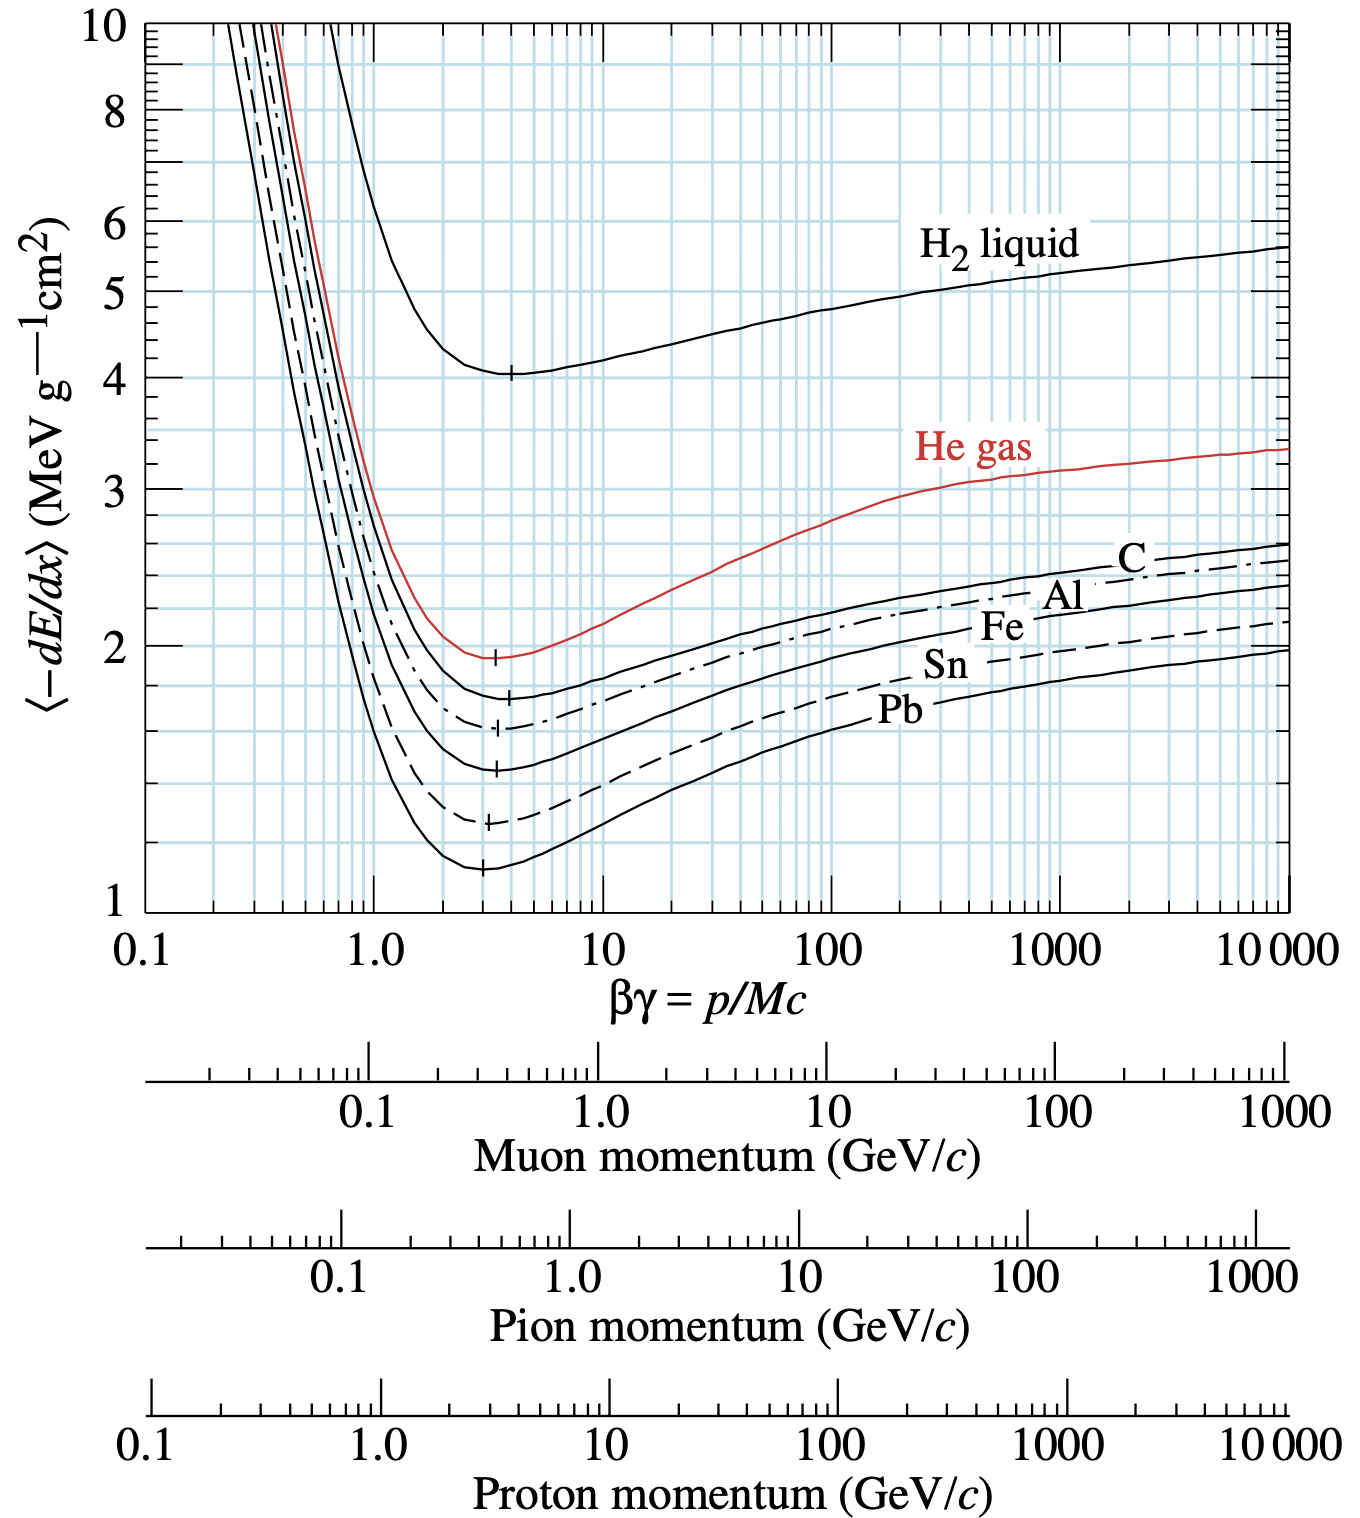
\includegraphics[keepaspectratio, scale=0.4]
 	{Figure/Siwecal/dedx.png}
 		\caption{水素(液体)、ヘリウム(気体)、炭素、アルミニウム、鉄、スズ、および鉛における平均エネルギー損失と、入射粒子(ミューオン、パイ中間子、陽子)の速度の関係。}
		 \label{dedx}
	\end{center}
 \end{figure}
\subsubsection{制動放射}
荷電粒子が物質を通過する際には電離の他に、原子核との衝突によって電磁波を放射しエネルギーを失うこともある。物質を構成する原子核はそれぞれ電場を持っており、電場によってRutherford散乱を受けた荷電粒子は加速、減速をされ、光子を放射しエネルギーを失う。これを制動放射と呼ぶ。制動放射によって荷電粒子が失うエネルギー損失率は、
\begin{equation}
	\label{energyloss}
	- { \frac{dE}{dx} } = \frac{E}{L_R}
\end{equation}
$L_R$は放射長と呼ばれており、平均エネルギーが$e$の因子だけ小さくなる平均の長さを指す。$L_R$は近似的に以下のように与えられる。
\begin{align}
\frac{1}{L_R} = 4 {\left( \frac{\hbar}{mc} \right)}^2 Z (Z+1) {\alpha}^3 n_{\alpha} \ln\left(\frac{183}{Z^{1/3}}\right)
\end{align}
式(\ref{energyloss})を積分することで、初期エネルギー$E_0$を持った荷電粒子が物質を$x$だけ進むときのエネルギー損失は以下のようになる。
\begin{equation}
E = E_0 \exp(-x/L_R)
\end{equation}
電離エネルギーと制動放射によって失うエネルギーの大きさが同じになる入射電子のエネルギーを臨界エネルギー$E_c$と呼び、この値よりもエネルギーが小さい場合はエネルギー損失がBethe-Blochの式に従い、大きい場合は制動放射によって主にエネルギーを失う。(臨界エネルギーは物質によって異なるがおおよそ$E_c \simeq \SI{500}{MeV} / Z$と表される。)荷電粒子の制動放射によって失われるエネルギーは質量の二乗に反比例するが、電離エネルギー損失は質量に強く依らないため、ほとんどの粒子に対しては制動放射よりも電離損失が支配的となる。 一方で電子においては制動放射によるエネルギー損失が支配的であり、$E_c$は電磁カロリメータなどの設計において重要なパラメータとなる。
\subsection{光子}
電荷を持たない光子は物質中で電離は起こさず、主に図\ref{photon}に示す光電効果、コンプトン散乱、電子陽電子対生成の 3 つの過程で相互作用する。
\begin{figure}[H]
	\begin{center}
 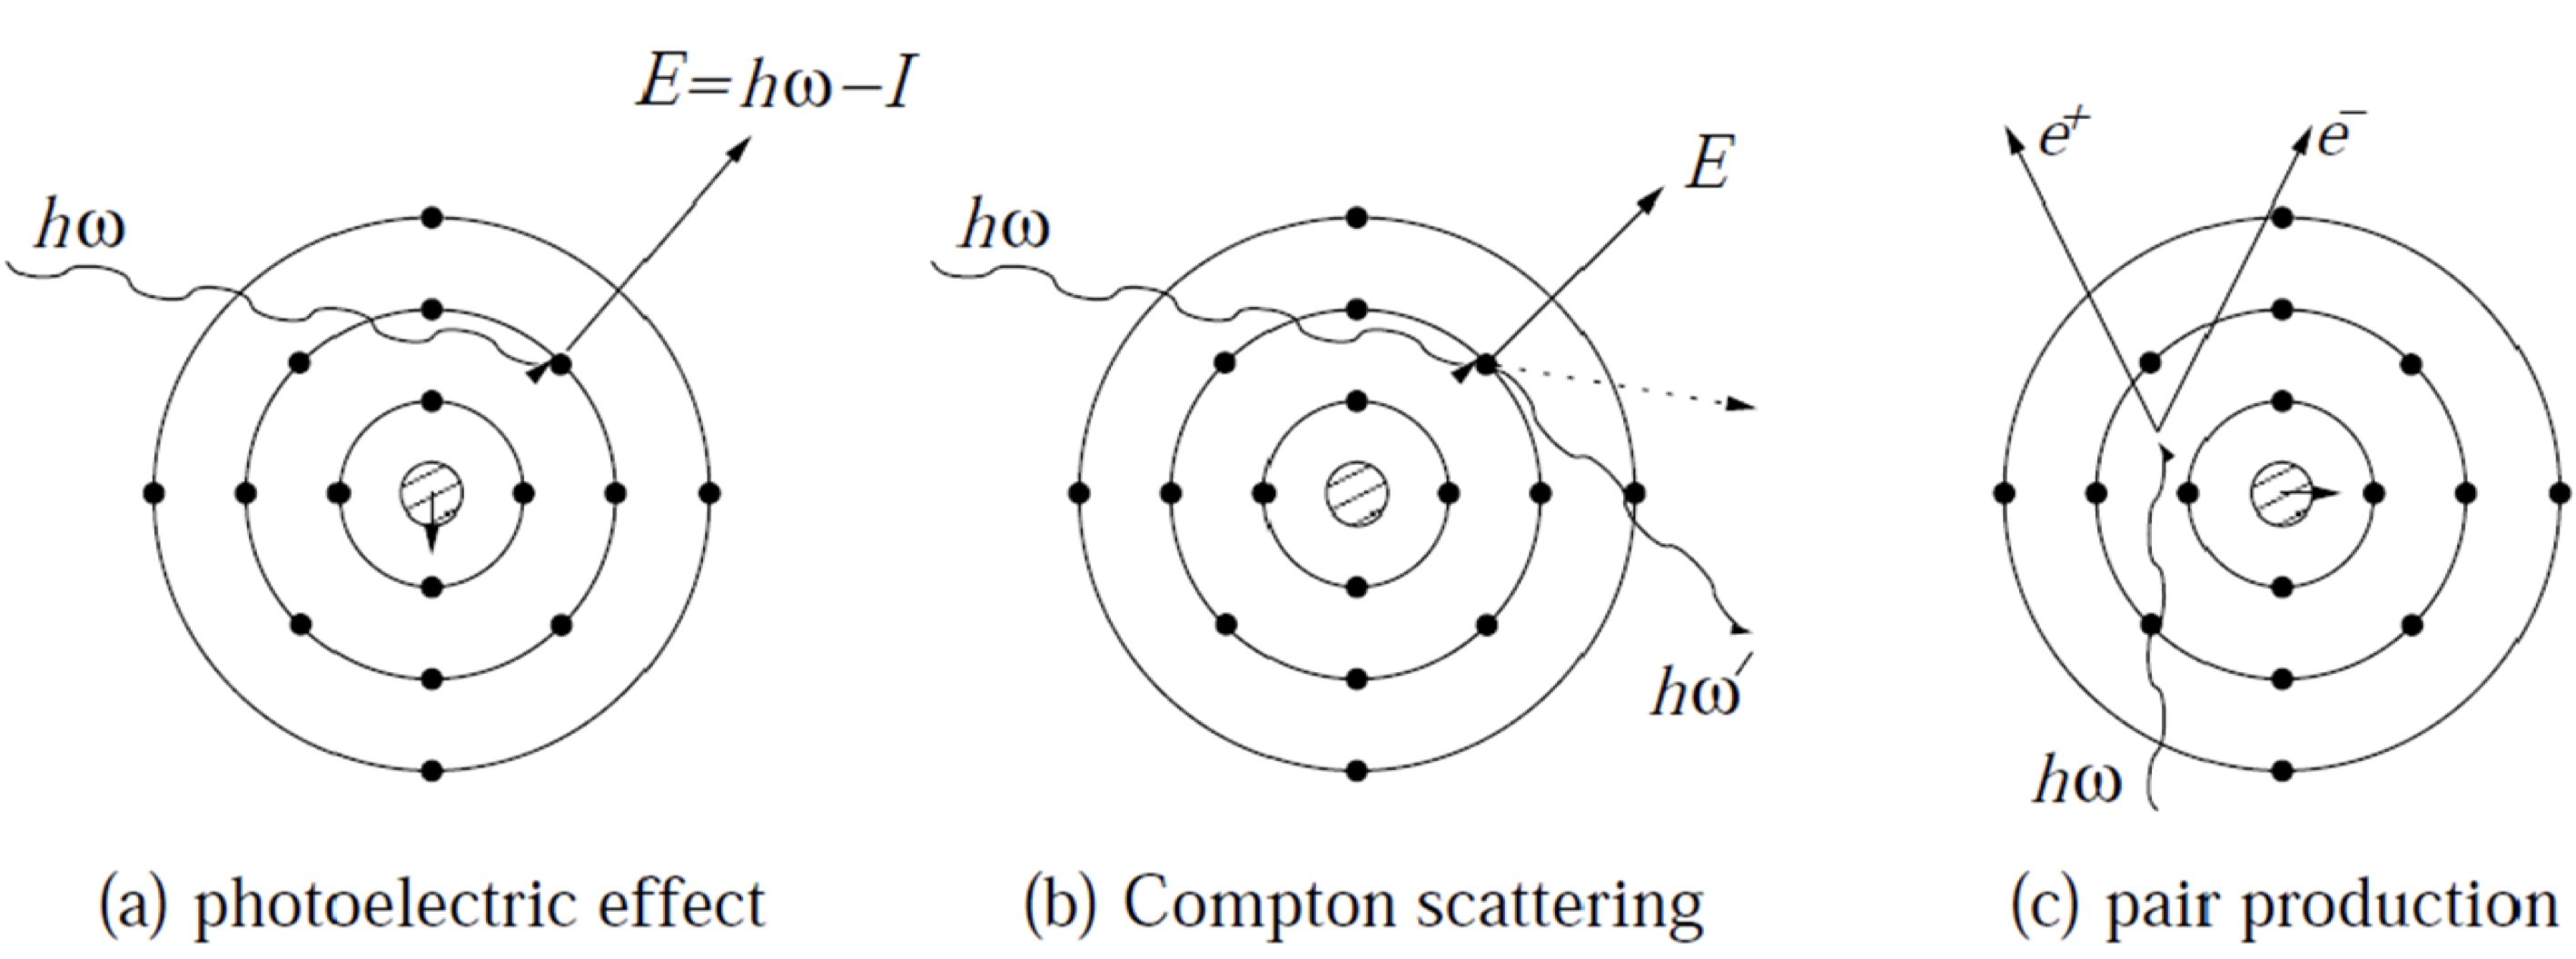
\includegraphics[keepaspectratio, scale =0.2]
 	{Figure/Siwecal/photon.png}
 		\caption{光子と物質の相互作用}
 		\label{photon}
	\end{center}
 \end{figure}
\begin{itemize}
 \item 光電効果 (Photoelectric effect): 入射光子が物質に当たることで光子の持っていたエネルギー$h\nu$が物質の電子に与えられる。これによって励起された電子が$h\nu - I$の運動エネルギーで飛び出す現象。($I$はイオン化エネルギー)
 \item コンプトン散乱 (Compton scattering): 入射光子と原子核に束縛されている1つの電子との弾性散乱。光電効果よりも光子のエネルギーが大きく、電子陽電子対生成反応よりも小さい時に支配的な反応である。
 \item 電子陽電子対生成 (Pair production): 入射光子が原子核のつくるクーロン場において消滅し、電子陽電子の対を生成する反応。この反応では、光子のエネルギーが電子陽電子の静止質量の和(およそ$\SI{1.02}{MeV}$)よりも大きい必要がある。
\end{itemize} 
 光子のエネルギーによってこれらの反応確率は異なり、図\ref{photon_cs}に光子のエネルギーに対する各反応の確率を示す。中でも数MeV 以上の光子においては電子陽電子生成反応が主要なプロセスであり、ILCのような高エネルギーにおいては電子陽電子対生成が重要である。 物質に入射した光子は電子陽電子を生成し、さらに制動放射によって光子を放出する。これを繰り返すことで電子陽電子と光子の数が指数関数的に増加していき、この現象が電磁シャワーと呼ばれている。この時、電子陽電子対生成過程の断面積は$E_\gamma \gg mc^2/ \alpha Z^{1/3}$において
 \begin{align}
 \sigma_{pair} = \frac{7}{9}\frac{1}{n_a L_R}
 \end{align}
 と近似することができ、光子の飛程はおよそ9/7\, $L_R$となる。電磁シャワーは発展するにつれて光子の平均エネルギーが下がり、臨界エネルギー(ILCの検出器ではおよそ\SI{10}{MeV})に到達すると電子陽電子生成過程が起こらなくなり終息する。粒子のエネルギーを測定する場合には、シャワー内の荷電粒子をMIPとみなし、それらの粒子数が初めの光子のエネルギーに比例すると考えることで、検出器のセンサーに残したエネルギー損失の和をとることで測定する。

また電磁シャワーは進行方向だけでなく垂直方向にも広がり、モリエール半径$R_M$によって広がりが特徴づけられる。モリエール半径とは、エネルギーの90$\%$が入るシャワーの半径を指し、以下の式で表される。
\begin{equation}
 \label{moliere}
 R_M \sim \frac{21 (\mathrm{MeV}) L_R}{臨界エネルギー (\mathrm{MeV})}  (\mathrm{g}/\mathrm{{cm}^2})
\end{equation}
\begin{figure}[h]
	\begin{center}
 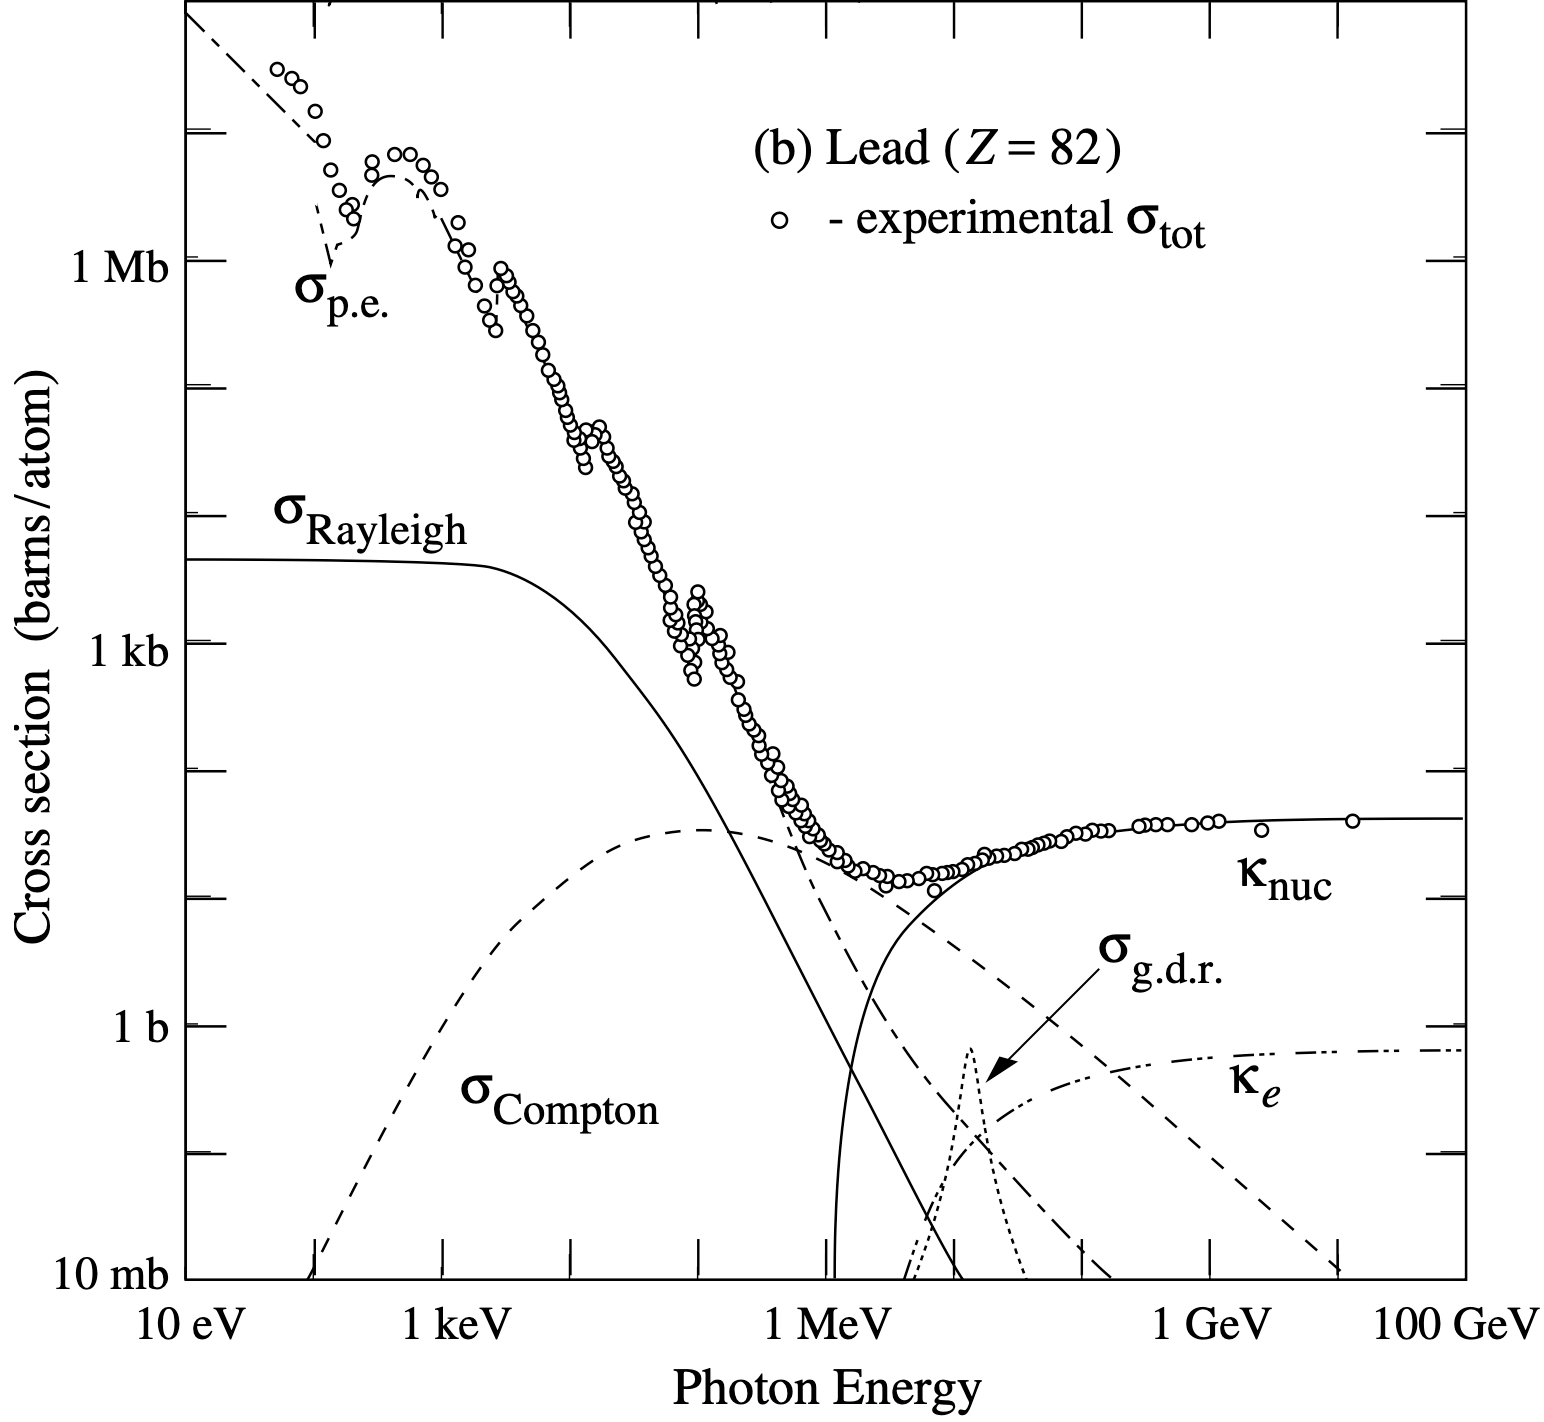
\includegraphics[keepaspectratio, scale=0.4]
 	{Figure/Siwecal/photon_crosssection.png}
 		\caption{光子と鉛の相互作用における断面積と光子のエネルギーの関係。${\sigma}_{p.e.}$は光電効果を、${\sigma}_{Compton}$はコンプトン散乱を、${\kappa}_{e}, {\kappa}_{nuc}$は電子陽電子対生成を指す。}
 		\label{photon_cs}
	\end{center}
 \end{figure}
\subsection{ハドロン}
$\pi$中間子やK中間子などのハドロンは物質を構成する原子核と衝突し、非弾性散乱を繰り返すことでハドロンシャワーを生成する。ハドロンの相互作用長は典型的に放射長よりも大きく、ハドロンをカロリメータで測定する場合には非常に多くの物質を必要とする。相互作用長は以下のように表される。
\begin{align}
\lambda = \frac{A}{N_a \rho} \sigma_{total}
\end{align}
ここで、$\rho$は物質の密度を、$ \sigma_{total}$は反応断面積の総和を表す。ハドロンシャワーには${\pi}^0 \rightarrow \gamma \gamma$崩壊によって発生する電磁シャワーが混ざってしまっており、検出器のエネルギー応答が異なることから、ハドロンシャワーのエネルギー分解能は電磁シャワーと比較して非常に悪くなってしまう。

\section{粒子検出器の動作原理}
 素粒子実験では、前節の相互作用を用いて粒子を検出する。粒子の検出には、事象を区別するために十分な時間分解能と位置分解能を持つ必要があり、また各粒子を識別するために、エネルギーと運動量を十分な精度で測定する必要がある。以下では、測定器を構成する検出器のうち特に重要なものを取り上げる。

\subsection{ガス検出器}
 ガス検出器は、主にアルゴンのような活性の低いガスを検出器内に充填した検出器である。荷電粒子がガス中を通過することで電離反応を起こし、生成される電子と陽イオンを電極に集める、あるいは電離の軌跡を可視化することで荷電粒子を検出することができる。主な検出器としては、電極への印加電圧が小さい領域では電離箱が、大きい領域ではワイヤーチェンバーやRPCなどが挙げられる。

\subsection{半導体検出器}
 半導体検出器とは半導体材料を使用した検出器を指し、光や電子をはじめとして様々な粒子を検出するものがある。半導体材料には主にシリコンやゲルマニウムが用いられ、接合ダイオードの原理を使用して製造される。以下では、シリコン検出器の構造と動作原理について説明する。まず基本構造としては、検出器の一方に正孔の多いp型半導体、もう一方の面に自由電子が多いn型半導体のp-n接合が作られてある。それぞれに対して逆バイアス電圧(p型に負、n型に正)を印加することで、p型とn型との間で正孔と自由電子の結合が進み、空乏層と呼ばれる安定化した領域が検出器の接合面を中心に広がる。この空乏層を通過した荷電粒子は、検出器内のシリコン原子を励起し、電子正孔対を生成する。飛跡に沿って生成された電子正孔対は、空乏層内の電場によって両印加極板までドリフトされ、パルス電流として測定される。また、シリコンなど半導体のバンドギャップは1eV程度であり、電子正孔対を生成するために必要なエネルギーはおよそ$3,4$eVとなっている。この信号の小ささから、半導体検出器では読み出しにおいて増幅を必要とするため、増幅回路が近傍(あるいは半導体内部)に存在している。半導体検出器は、電極が平面構造のピクセル検出器や帯状のストリップ検出器、検出器基板上に増幅回路を形成するモノリシック検出器など、電極や増幅回路の実装によって様々な構造が存在する。

\subsection{シンチレーション検出器}
 励起エネルギーの一部が、より低いエネルギー準位へ遷移する際に可視光として表れる物質をシンチレータという。シンチレータ検出器は、荷電粒子の通過によって発生した蛍光(シンチレーション光)を光検出器によって測定することで動作する検出器である。シンチレーション光は非常に弱い光信号であるため、光電子増倍管や半導体光センサーなどを用いて信号を検出する。
 
\section{シリコンタングステン電磁カロリメータ SiW-ECAL}
\subsection{SiW-ECALの全体構造}
ILDのSiW-ECALは、図\ref{SiW-ECAL}のようにタングステンの吸収層とシリコンパッドセンサーの検出層が、30層サンドウィッチ状に交互に重なったサンプリング型カロリメータである。1つのモジュールが10ほどのサブモジュールに分かれており、サブモジュールにはそれぞれ4枚のシリコン半導体センサーが貼り付けられる。
\begin{figure}[h]
 \begin{minipage}[h]{.45\linewidth}
	\begin{center}
 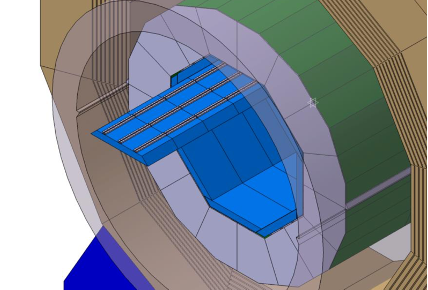
\includegraphics[keepaspectratio, scale=0.8]
 	{Figure/Siwecal/ECAL.png}
 		\caption{ILDおよびECALの全体図\cite{tdr2}}
 		\label{ECAL}
	\end{center}
\end{minipage}
\hfill
\begin{minipage}[h]{.45\linewidth}
	\begin{center}
 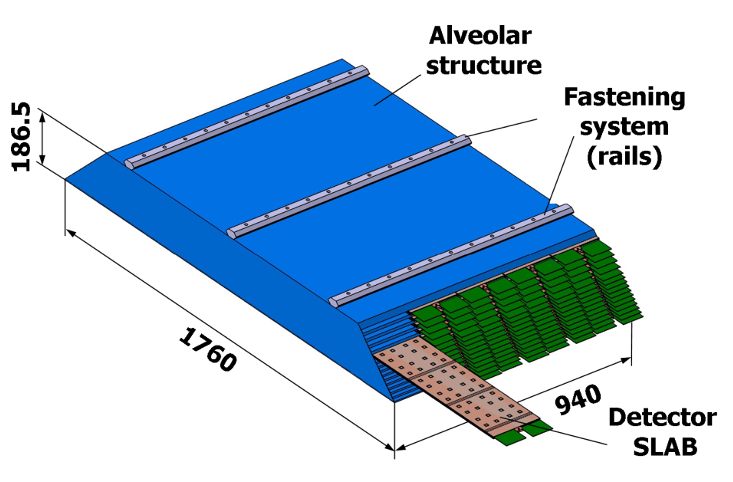
\includegraphics[keepaspectratio, scale=0.8]
 	{Figure/Siwecal/SiW-ECAL.png}
 		\caption{SiW-ECALの構造}
 		\label{SiW-ECAL}
	\end{center}
\end{minipage}
\end{figure}

\subsection{シリコン半導体検出器}
SiW-ECALでは検出層にシリコン半導体検出器を用いる。センサーの大きさは1枚あたり$9 \times 9\: \mathrm{{cm}^2}$で、1枚に$5.5 \times 5.5\: {\mathrm{mm}^2}$のピクセルが$16 \times 16$個並んでおり、1つのサブモジュールあたり1024チャンネル読み出しが可能となっている。またシリコンセンサーには、電極としてアルミニウム ($\mathrm{Al}$) 、絶縁層に二酸化ケイ素 ($\mathrm{SiO_2}$)が使用される。 厚さ320$\mathrm{\mu m}$のセンサーでは、1MIPあたり$\SI{86.8}{keV}$のエネルギー損失が起こり、臨界エネルギーに達するまでに生成される電子正孔対はおよそ24,000、電荷にして$\SI{4}{fC}$となる。シリコンセンサーは、常温硬化型導電性接着剤によって回路基板(PCB)と接着されており、PCBを通して信号の読み出しが行われる。以下にセンサーの仕様と1枚のシリコンセンサーパッドを示す。
\begin{figure}[H]
 \begin{minipage}[h]{.45\linewidth}
 \def\@captype{table}
   \centering
   \tblcaption{シリコンセンサーの仕様}
   \begin{tabular}{|c|c|}
         \hline
   	制作会社 & 浜松ホトニクス株式会社\\
	サイズ & 89.7 $\times \SI{89.7}{mm}^2 $ \\
	セルサイズ & 5.5 $\times \SI{5.5}{mm}^2 $\\
	セル数 & 16 $\times$ 16 = 256\\
	厚さ & 320/500/$\SI{650}{}$\\
	完全空乏化電圧 & 40/70/$\SI{110}{V}$\\
        \hline
  \end{tabular}
\end{minipage}
\hfill
\begin{minipage}[h]{.45\linewidth}
	\begin{center}
 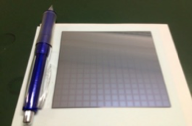
\includegraphics[keepaspectratio, scale=0.8]
 	{Figure/Siwecal/si_sensor.png}
 		\caption{シリコンパッドセンサー}
 		\label{sensor}
	\end{center}
\end{minipage}
\end{figure}
\subsection{読み出しシステム}
 SiW-ECALは高精細であることから読み出しチャンネル数が非常に多くなっており、30層のECAL全体ではおよそ1億にもおよぶ。そのため、シリコンセンサーからの信号読み出しをコンパクトにする必要があり、読み出し専用のApplication Specific Integrated Circuit (ASIC) が開発された。現在の技術プロトタイプに実装されているASICには、フランスのOmegaグループが開発した Sillicon Kalorimeter Integrated ReadOut Chip (SKIROC) シリーズの第二バージョンであるSKIROC2Aを用いている。\\
 まず、読み出しに用いるASICに求められる性能には次に挙げる項目が求められる。
 \begin{itemize}
	\item 自動トリガー:\\
		信号に対してASIC自身でトリガーをかける。
	\item 完全デジタル出力:\\
		 シリコン半導体検出器からのアナログ情報をすべてデジタル変換し、データ量を圧縮してData AcQuisition (DAQ)へ送信する。
	\item 発熱量の抑制 :\\
		電力消費によって発生するジュール熱を、1チャンネルあたり25$\mathrm{\mu W}$ 以下に抑える。
	\item 1 MIP 相当の信号を識別できる高い Signal to Noise 比 (S/N 比):\\
		PFAにおいてジェットエネルギー分解能を向上させるために、高い精度でノイズからシグナルを分離する必要がある。
 \end{itemize}
 続いて、SKIROC2Aの基本的な仕様を以下に示し、図\ref{skiroc2a}にSKIROC2Aのアナログ部の回路図を示す。
 \begin{itemize}
 	\item Austria Micro Systems社製 $\SI{0.35}{\mu m}$ SiGe
	\item 7.5 $\times \SI{8.5}{mm^2} /1チップ$
	\item 1チップあたり64チャンネル読み出し可能
	\item 2種類のダイナミックレンジをもつ Analog to Digital Converter (ADC) mode :\\
		電磁シャワー内の粒子が1つのチャンネルに大量に入射したときに全エネルギーを測定出来るよう、幅広いゲインのレンジを持つ。
		\begin{itemize}
			\item High gain \ldots \ 0.5 $\sim$ 150 MIP 相当の信号に対応
			\item Low gain \ldots \ 150 $\sim$ 2500 MIP 相当の信号に対応
		\end{itemize}
	\item TDC (Time to Digital Converter) mode : $\SI{1}{ns}$程の時間分解能で時間情報を保存
	\item 1チャンネルあたり15イベント保持可能なAnalog memory cell\\
		ビームバンチ構造に対応するため、$\SI{200}{ns}$の間イベントを保持することが可能。1つのMemory cellでは、High gain ADC、Low gain ADCを、時間情報であるBunch crossing ID (BCID) と紐づけて保存。
	\item 数珠つなぎ型読み出し : 順番に読み出すことで読み出していないチップの電源を必要とせず、消費電力を減らす
	\item 0.5 MIPでの自動トリガー
	\item 全64チャンネルの閾値を個別で同時設定可能な$\SI{10}{bit}$ Digital Analog Converter (DAC) threshold
	\item Power pulsing mode
 \end{itemize}
データ収集の手順は、以下のとおりである。まずシリコンセンサーからのアナログ信号が各チャンネルに入力され、前置増幅器によって前段増幅を行う。ここでの増幅率は、前置増幅器のfeedback capacitanceによって変更可能となっており、増幅率が最大となる$\SI{0}{pF}$から$\SI{6.0}{pF}$まで$\SI{0.4}{pF}$刻みで決定することができる。前段増幅を経た信号は、Fast shaperと2つのSlow shaper(Low/High gain)の3つに分割される。Fast shaperに入った信号は、CRRC shaperによって信号をさらに増幅したのち、discriminatorにて閾値を超えた場合のみトリガー信号を出し、同時に入ってきたSlow shaperの信号電圧をMemory cellに保持する。ここで、CRRC shaperとは微分回路と積分回路を組み合わせた回路であり、信号増幅率と立ち上がり時間を調整している。Memory cell に保持された電荷は、読み出し時間が経過、あるいはMemory cellが満たされたタイミングでマルチプレクサー(MUX)に送られる。一方、Slow shaperにおいても信号がCRRC shaperによって増幅率1、10倍に増幅され、トリガー信号によってMUXに送られる。MUXでは、Slow shaper(Low or High)とTDCの組み合わせを決定し、Wilkinson型$\SI{12}{bit}$ ADCによってアナログ信号をデジタル化し、メモリに保存されたのち外部へ転送される。
\begin{figure}[H]
	\begin{center}
	\includegraphics[keepaspectratio, scale=0.7]
% 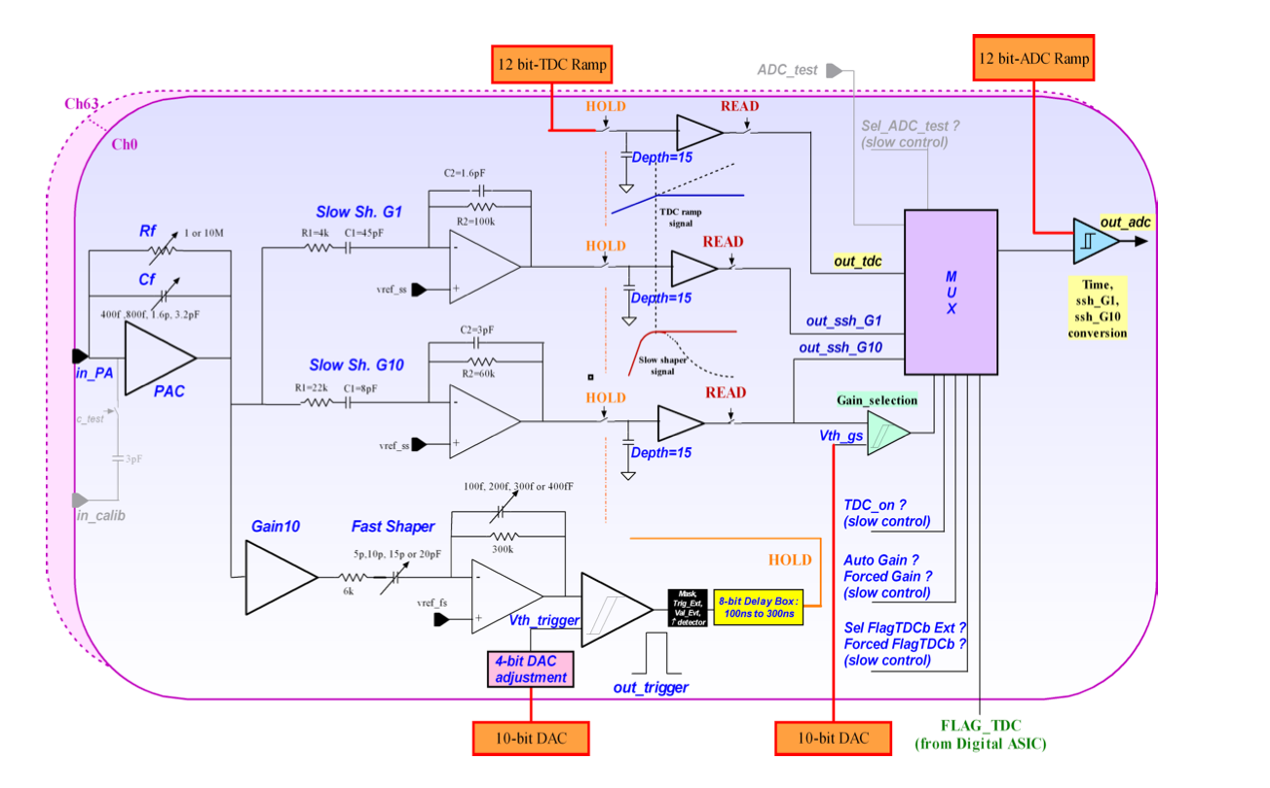
\includegraphics[width=\linewidth,angle=90, scale=1.5]
 	{Figure/Siwecal/skiroc2A.png}
 		\caption{SKIROC2Aのアナログ部の回路図}
 		\label{skiroc2a}
	\end{center}
 \end{figure}

\subsection{タングステン吸収層}
ILDのSiW-ECALの吸収層ではPFAの要件を満たすために、相互作用長が長く放射長の短い物質でシャワーの広がりを小さく抑える物質を採用する必要がある。そのため、モリエール半径が小さく、放射長に比べ相互作用長が大きいタングステンが採用されている。表\ref{metal}に物質量が大きく吸収層の候補となる物質の性質について示す。
\begin{table}[h]
 \centering
  \begin{tabular}{c||SSS}
   \hline
   物質 & $\lambda/\mathrm{cm}$ & $L_R/\mathrm{cm}$ & $R_M/ \mathrm{cm}$ \\
   \hline \hline
	鉄 & 16.8 & 1.76 & 1.69\\
	銅 & 15.1 & 1.43 & 1.52\\
	タングステン& 9.6 & 0.35 & 0.93\\
	鉛 & 17.1 & 0.56 & 1.00\\
   \hline
  \end{tabular}
   \caption{物質量の大きい吸収層の候補物質($\lambda$は相互作用長、$L_R$は放射長、$R_M$はモリエール半径を示す。)}
   \label{metal}
\end{table}
\subsection{技術プロトタイプ}
SiW-ECALの技術プロトタイプとして、図\ref{shortslab}のような構造が考えられている。図\ref{shortslab}は、1層の検出器 (Slab) の一部として作製されたShort slabである。図の上から構造体として炭素繊維強化プラスチック (CFRP) の板があり、その下に読み出し基板(FEV)やASICの制御基板があり、基板下にはセンサーに接触し電荷を印加する導電性シートがあり、さらにカーボンの板で挟まれている。1層あたり、FEVにはPCB上にSKIROC2Aが16チップ実装されており、裏面にはシリコンパッドセンサー4枚が導電性接着剤で接着されている。また、ASICはFPGAを通して制御されており、さらに図\ref{core}のに示すモジュールを通して、複数のSlabからの信号を同時に読み出している。

読み出し基板には、大きく分けてFEVとCOBの2つの案がある。(図\ref{fevcob})FEVはPCBの裏面に4枚のシリコンセンサーを導電性接着剤で接着しており、その内側にフレキシブル基板を接着することでシリコンセンサーへの電圧供給を行う。またPCB表面にはASICが16chip実装されており、センサーからの信号をデジタル変換している。FEVにはFEV7から13までのバージョンがあり、内部配線や外部接続の面でアップデートが行われている。一方でCOB (Chip On Board) では、ASICが窪みにワイヤーボンディングされており、これによって読み出し基板がFEVよりも薄いコンパクトな構造になっている点が特徴である。しかし同時に、FEVと比較してノイズの影響を受けやすいなど欠点も抱えている。

これら技術プロトタイプの開発は、フランスと日本を中心にCALICEグループによって国際協力で行われている。CALICE (Calorimeter for Linear Collider Experiment) はILCに向け、カロリメータの共同開発を目的として結成された国際コラボレーションであり、九州大学のグループもこの一員である。また、モジュールの生産・組み立ては国内においても可能となっている。
\begin{figure}[h]
	\begin{center}
	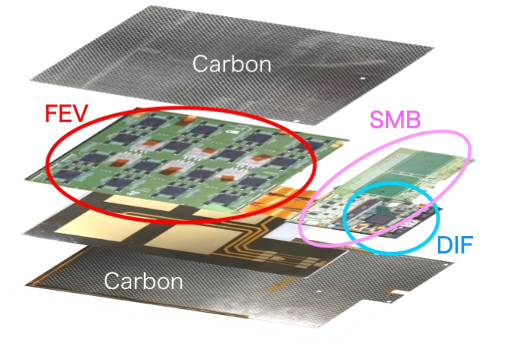
\includegraphics[keepaspectratio, scale=0.7]
 	{Figure/Siwecal/shortslab.png}
 		\caption{short slabの構造}
 		\label{shortslab}
	\end{center}
 \end{figure}
 \begin{figure}[ht]
	\begin{center}
	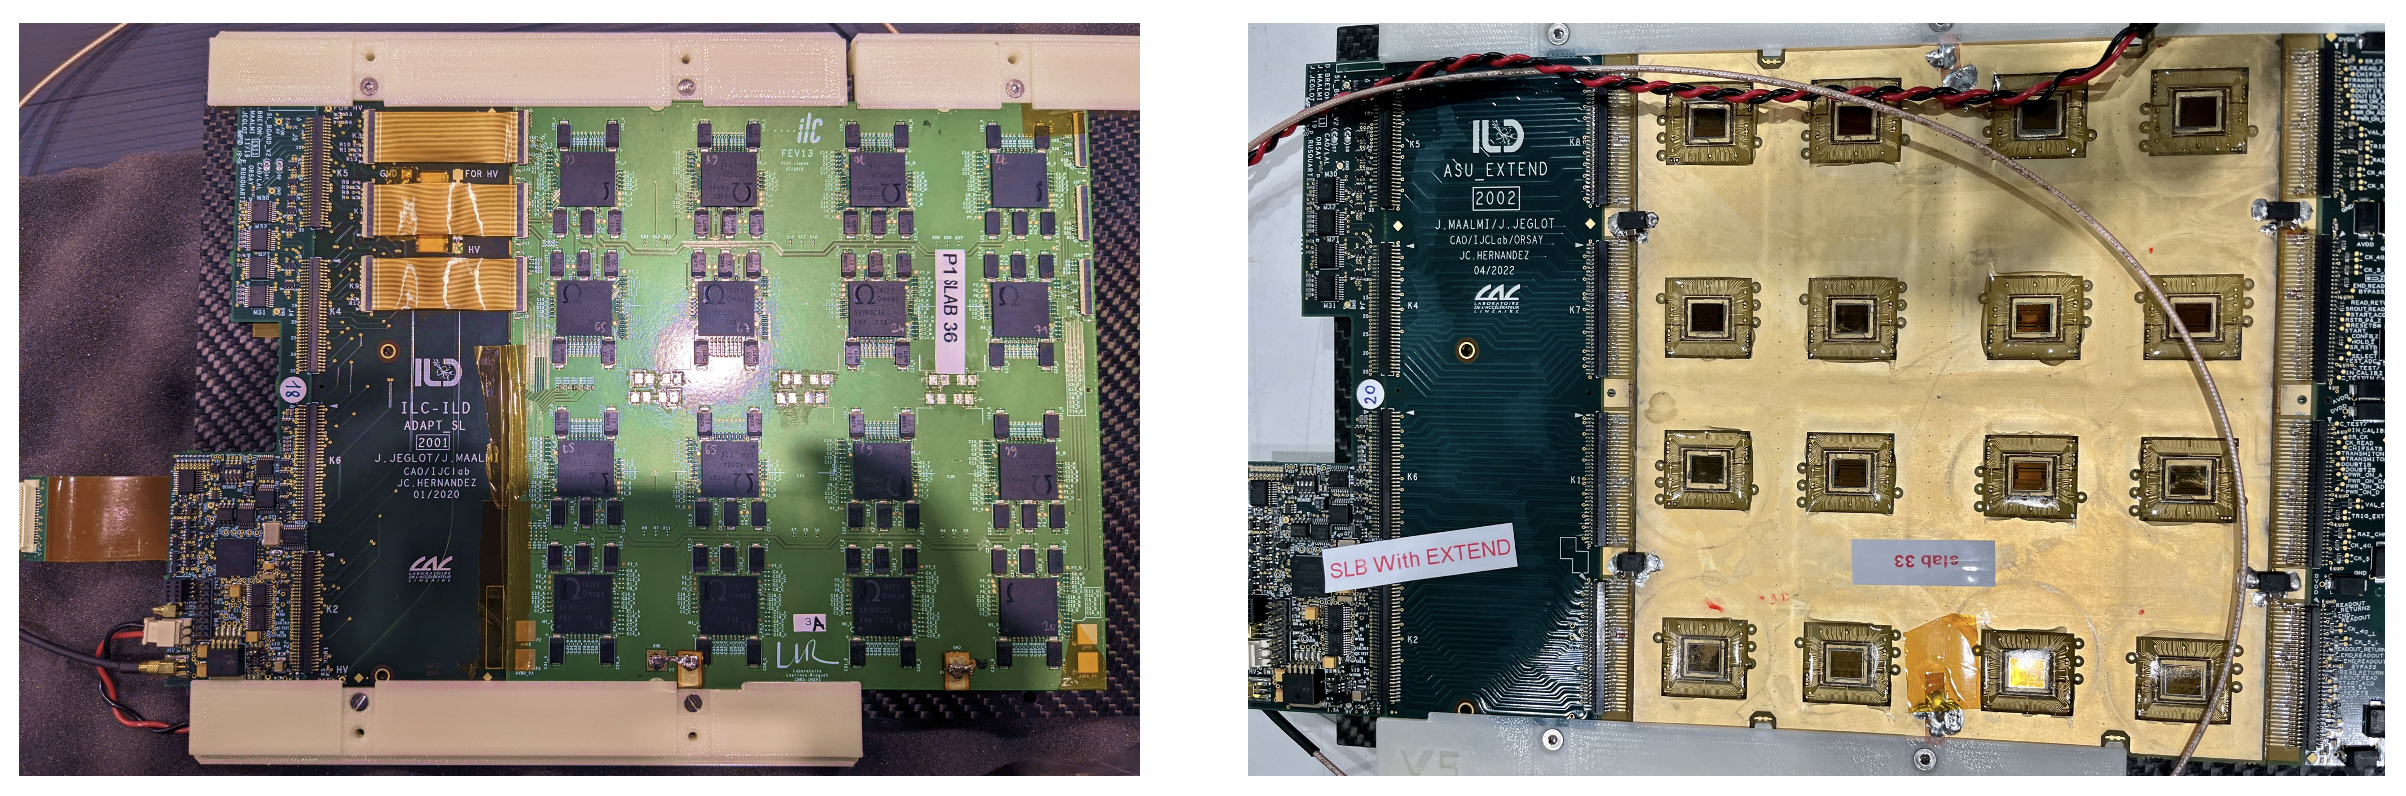
\includegraphics[keepaspectratio, scale=0.3]
 	{Figure/Siwecal/fevcob.png}
 		\caption[FEV13, COB]{(左) FEV13 (右) COB}
 		\label{fevcob}
	\end{center}
 \end{figure}
 \begin{figure}[ht]
	\begin{center}
	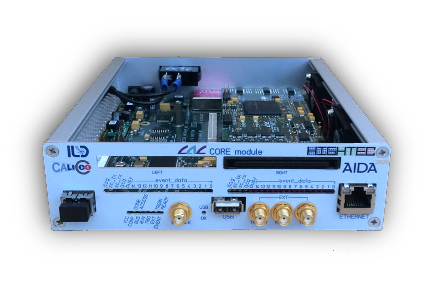
\includegraphics[keepaspectratio, scale=0.7]
 	{Figure/Siwecal/core.png}
 		\caption{多層読み出しのためのCOREモジュール}
 		\label{core}
	\end{center}
 \end{figure}